\documentclass[12pt,a4paper]{article}

% --- Paquetes ---
\usepackage[utf8]{inputenc}
\usepackage[T1]{fontenc}
\usepackage[english]{babel}
\addto\captionsenglish{
  \renewcommand{\contentsname}{Índice}
  \renewcommand{\figurename}{Figura}
  \renewcommand{\tablename}{Tabla}
  \renewcommand{\refname}{Referencias}
}
\usepackage{lmodern}
\usepackage{geometry}
\geometry{margin=2.5cm}
\usepackage{fancyhdr}
\usepackage{amsmath}
\usepackage{graphicx}
\usepackage{float}
\usepackage{booktabs}
\usepackage{array}
\usepackage{xcolor}
\usepackage{listings}
\usepackage{titlesec}
\usepackage{hyperref}
\usepackage{enumitem}
\usepackage{caption}
\usepackage{subcaption}
\usepackage{parskip}

% --- Colores UPS ---
\definecolor{salesiana}{RGB}{0,84,166}
\definecolor{accentgreen}{RGB}{34,139,34}
\definecolor{accentorange}{RGB}{204,85,0}
\definecolor{codebg}{RGB}{245,245,245}

% --- Código ---
\lstdefinestyle{cppstyle}{
  backgroundcolor=\color{codebg},
  basicstyle=\ttfamily\footnotesize,
  keywordstyle=\color{salesiana}\bfseries,
  commentstyle=\color{accentgreen}\itshape,
  stringstyle=\color{accentorange},
  breaklines=true,
  frame=single,
  rulecolor=\color{gray!40},
  numbers=left,
  numberstyle=\tiny\color{gray},
  language=C++,
  literate={á}{{\'a}}1 {é}{{\'e}}1 {í}{{\'i}}1 {ó}{{\'o}}1 {ú}{{\'u}}1
           {ñ}{{\~n}}1 {Á}{{\'A}}1 {É}{{\'E}}1 {Í}{{\'I}}1 {Ó}{{\'O}}1
           {Ú}{{\'U}}1 {Ñ}{{\~N}}1
}
\lstdefinestyle{pystyle}{
  backgroundcolor=\color{codebg},
  basicstyle=\ttfamily\footnotesize,
  keywordstyle=\color{salesiana}\bfseries,
  commentstyle=\color{accentgreen}\itshape,
  stringstyle=\color{accentorange},
  breaklines=true,
  frame=single,
  rulecolor=\color{gray!40},
  numbers=left,
  numberstyle=\tiny\color{gray},
  language=Python,
  literate={á}{{\'a}}1 {é}{{\'e}}1 {í}{{\'i}}1 {ó}{{\'o}}1 {ú}{{\'u}}1
           {ñ}{{\~n}}1 {Á}{{\'A}}1 {É}{{\'E}}1 {Í}{{\'I}}1 {Ó}{{\'O}}1
           {Ú}{{\'U}}1 {Ñ}{{\~N}}1
}
\lstset{style=cppstyle}

% --- Títulos ---
\titleformat{\section}{\large\bfseries\color{salesiana}}{}{0em}{}[\titlerule]
\titleformat{\subsection}{\normalsize\bfseries\color{salesiana!80}}{}{0em}{}

% --- Encabezado/pie ---
\pagestyle{fancy}
\fancyhf{}
\lhead{\small\color{gray}Universidad Politécnica Salesiana}
\rhead{\small\color{gray}Visión por Computador · Práctica 4-1}
\cfoot{\thepage}
\renewcommand{\headrulewidth}{0.4pt}

\hypersetup{colorlinks=true, linkcolor=salesiana, urlcolor=salesiana, citecolor=salesiana}

% =============================================================================
\begin{document}
% =============================================================================

% --- Portada ---
\begin{titlepage}
  \centering
  \rule{\linewidth}{1.5pt}\\[0.4cm]
  {\large\bfseries UNIVERSIDAD POLITÉCNICA SALESIANA}\\[0.1cm]
  {\normalsize CARRERA DE INGENIERÍA EN CIENCIAS DE LA COMPUTACIÓN}\\[0.2cm]
  \rule{\linewidth}{0.8pt}

  \vspace{2cm}

  \parbox{0.85\textwidth}{\centering\LARGE\bfseries\color{salesiana}
    Clasificación de Objetos Usando Técnicas de Deep Learning: Fine-Tuning
    empleando YOLO y Ejecución de Redes de Detección de Objetos y
    Super Resolución en GPU
  }

  \vspace{1.5cm}

  {\large\bfseries Informe de Práctica 4-1 — Visión por Computador (G8)}\\[0.2cm]
  {\normalsize Práctica de Laboratorio — Unidad 4}

  \vspace{1.5cm}

  \begin{tabular}{ll}
    \textbf{Autores:}    & Michael Lata (Parte 1A, 1B, 1C) \\
                         & Jordy Romero (Parte 1A) \\[0.3cm]
    \textbf{Docente:}    & Vladimir Robles Bykbaev \\[0.3cm]
    \textbf{Asignatura:} & Visión por Computador \\[0.3cm]
    \textbf{Período:}    & Marzo -- Agosto 2026 \\[0.3cm]
    \textbf{Fecha:}      & 18 de julio de 2026 \\
  \end{tabular}

  \vspace{1cm}
  \parbox{0.8\textwidth}{\centering\small\itshape
    Las Partes 1B y 1C son de desarrollo individual y usan un equipo distinto
    (RTX 4060 Laptop, MAC propia) al de la Parte 1A, conforme lo exige la guía.
  }

  \vfill
  \rule{\linewidth}{1.5pt}
\end{titlepage}

% --- Resumen ---
\section*{Resumen}

Esta práctica tiene tres partes con distinto grado de individualidad según la guía. La Parte 1A (segmentación con YOLOv11, admite pareja) la hicimos en equipo junto a Jordy Romero: entrenamos YOLOv11n-seg por transferencia de aprendizaje sobre un dataset propio de tres clases (señal de pare, semáforo, cono de tránsito), y medimos una aceleración de 6.5x de GPU frente a CPU (99.0 FPS vs 15.2 FPS) en una RTX 3080.

Las Partes 1B y 1C son individuales y las hice íntegramente en mi propio equipo (RTX 4060 Laptop). En la Parte 1B comparé YOLOv12n y YOLOv26n para detección, y usé \textbf{RealPLKSR} (2024) en lugar de Real-ESRGAN (2021) para super resolución, porque la guía exige una red de no más de 2 años de antigüedad. Medí aceleraciones de 8.1x--8.7x en detección y 23.7x en super resolución. En la Parte 1C implementé un pipeline de preprocesamiento en OpenCV C++ (suavizado Gaussiano, morfología, Canny, ecualización de histograma) comparando una versión CPU pura contra una versión GPU-only, y obtuve 1.17x--1.74x de aceleración según la resolución de entrada.

\clearpage
\tableofcontents
\clearpage

% =============================================================================
\section{Introducción}
% =============================================================================

Esta práctica reúne tres tareas de visión por computador aceleradas por GPU: segmentación de objetos por transferencia de aprendizaje, comparación de redes de detección y super resolución en vídeo, y un pipeline clásico de preprocesamiento de imágenes en C++ con CUDA. El hilo conductor es el mismo en las tres partes: medir qué tan rápido corre una tarea en GPU frente a CPU, y entender \emph{por qué}.

La guía de práctica permite que la Parte 1A se resuelva en pareja, pero exige que las Partes 1B y 1C sean estrictamente individuales, con evidencia de un computador propio (dirección MAC única). Por eso esta práctica combina un trabajo en equipo (Parte 1A, junto a Jordy Romero) y un trabajo individual (Partes 1B y 1C, en mi propio equipo, distinto al de Jordy).

% =============================================================================
\section*{Repositorios del Proyecto}
% =============================================================================

\begin{itemize}
  \item \textbf{Parte 1A — Segmentación YOLOv11-seg (equipo Jordy Romero / Michael Lata):}\\
        \url{https://github.com/jordyromero03/ClasificacionObjetosYOLO}

  \item \textbf{Parte 1B y 1C — Trabajo individual (Michael Lata):}\\
        \texttt{Practica4-1 Michael Lata/} — repositorio git local, aún no publicado a un remoto.
\end{itemize}

% =============================================================================
\section{Parte 1A: Segmentación de Objetos con YOLOv11 (trabajo en equipo)}
% =============================================================================

\subsection{Dataset}

El dataset combina imágenes reales de COCO 2017 (val) para las clases con máscaras de segmentación poligonal ya disponibles, y conos de tránsito sintéticos generados con OpenCV para completar la tercera clase, dado que no se encontró un dataset público de conos con licencia adecuada y volumen suficiente:

\begin{table}[htbp]
  \centering
  \caption{Composición del dataset de Parte 1A}
  \begin{tabular}{llr}
    \toprule
    \textbf{Clase} & \textbf{Fuente} & \textbf{Anotaciones (train)} \\
    \midrule
    stop-sign     & COCO 2017 val (real)      & 52  \\
    traffic-light & COCO 2017 val (real)      & 448 \\
    traffic-cone  & Sintético (OpenCV)        & 103 \\
    \bottomrule
  \end{tabular}
  \label{tab:dataset1a}
\end{table}

La partición final quedó en 237 imágenes de entrenamiento, 53 de validación y 56 de prueba, en formato YOLO-segmentación (polígonos).

\subsection{Entrenamiento por transferencia de aprendizaje}

Usamos YOLOv11n-seg (Ultralytics) como base preentrenada y aplicamos fine-tuning de 60 épocas sobre el dataset propio:

\begin{lstlisting}[style=pystyle]
model = YOLO('models/yolo11n-seg.pt')
model.train(
    data='dataset_traffic/data.yaml',
    epochs=60, imgsz=640, batch=16, device=0,
    patience=15, lr0=0.001, lrf=0.01, momentum=0.937,
    weight_decay=0.0005, warmup_epochs=3,
    augment=True, degrees=10.0, fliplr=0.5, mosaic=1.0,
)
\end{lstlisting}

Entrenamos en el equipo de Jordy Romero (NVIDIA GeForce RTX 3080). No nos quedaron registradas las métricas de validación (mAP) de esta corrida del notebook; el análisis cuantitativo de esta sección se apoya en el benchmark de velocidad y en la inspección cualitativa de las inferencias, que sí guardamos.

\begin{figure}[htbp]
  \centering
  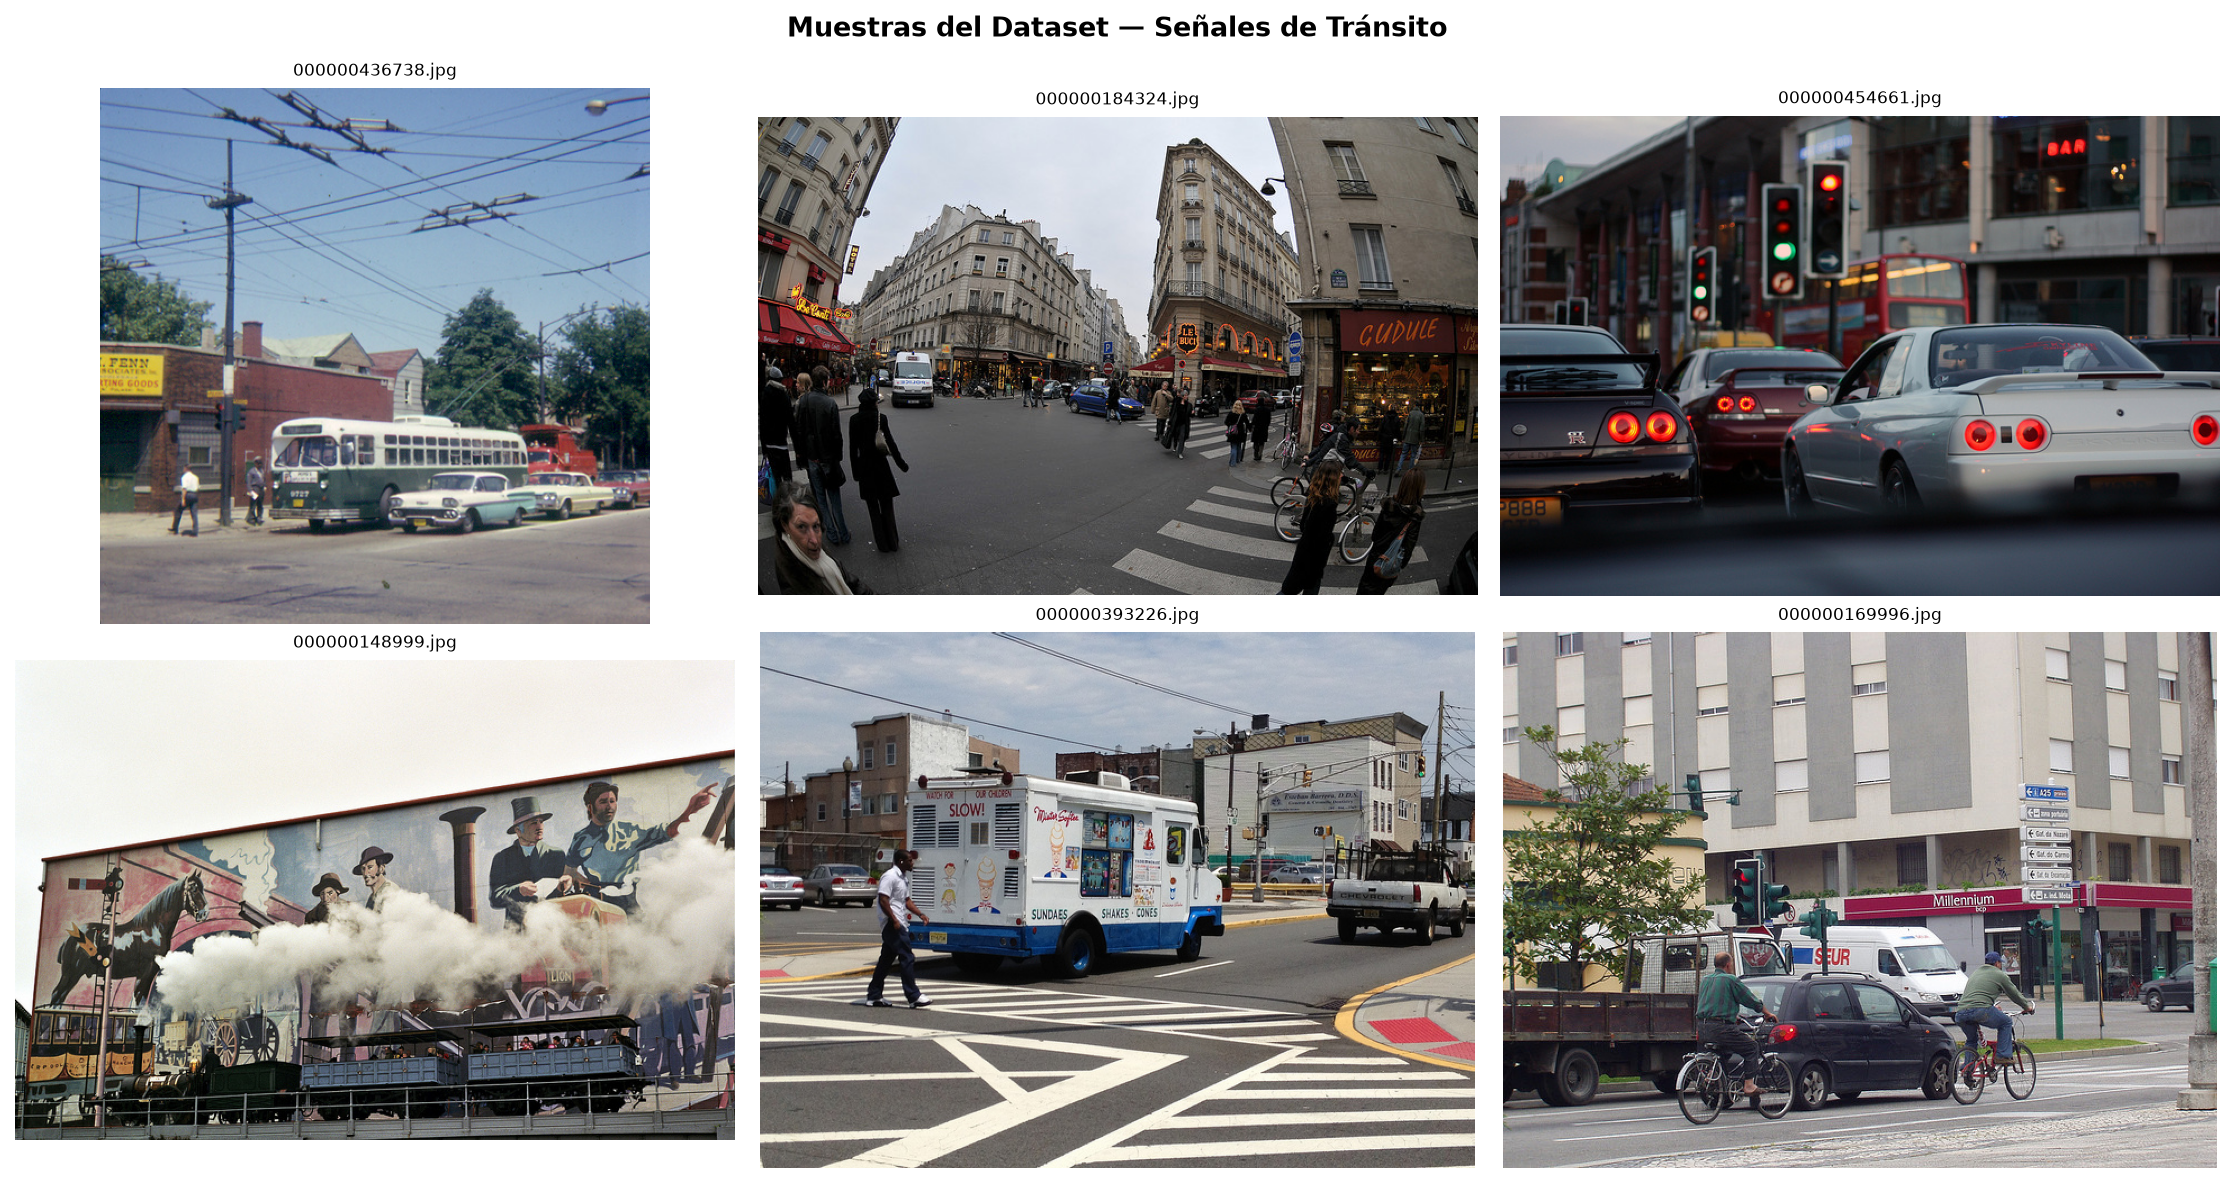
\includegraphics[width=0.85\textwidth]{capturas/dataset_samples.png}
  \caption{Muestras del dataset de entrenamiento: señales de pare, semáforos y conos de tránsito.}
  \label{fig:dataset1a}
\end{figure}

\subsection{Resultados}

\begin{figure}[htbp]
  \centering
  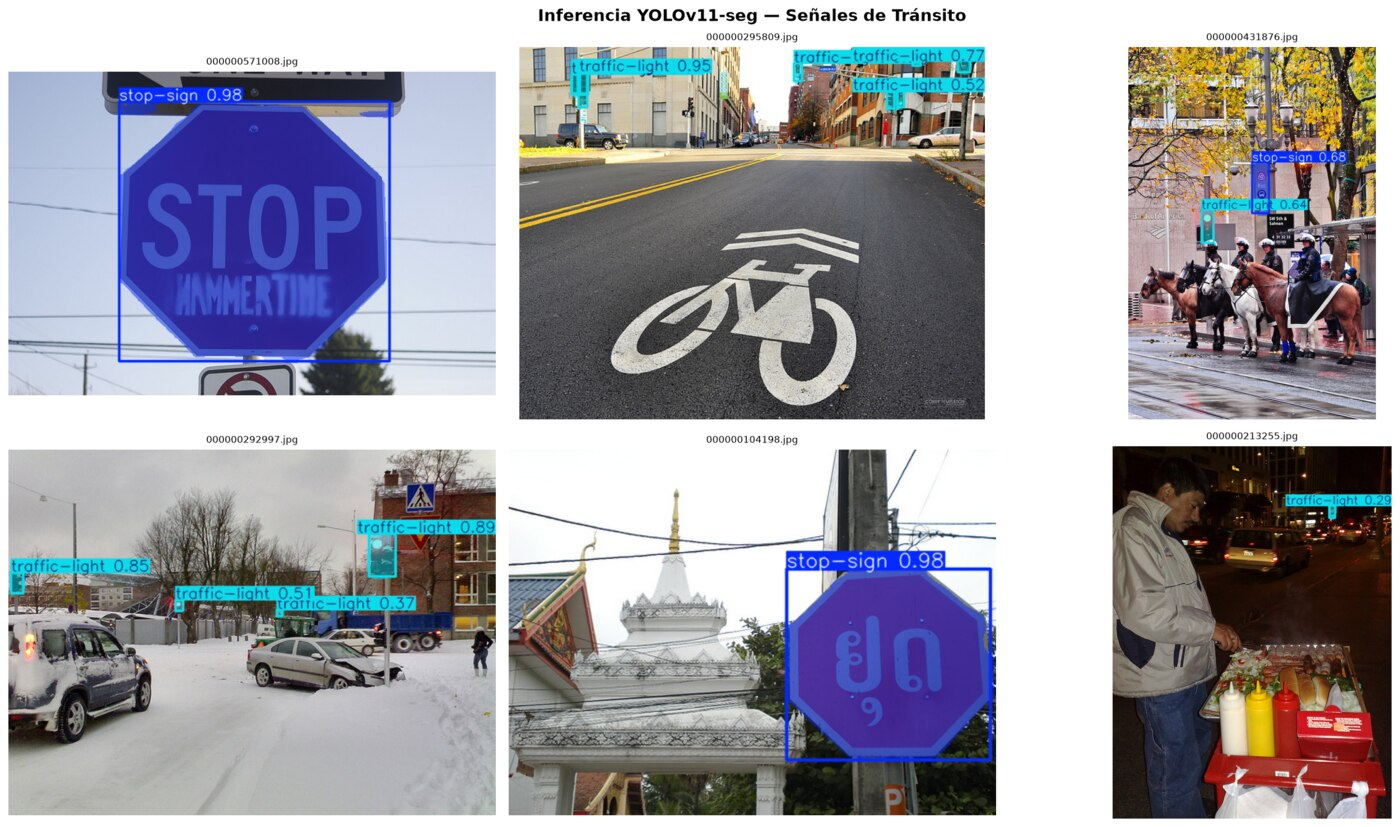
\includegraphics[width=0.85\textwidth]{capturas/inferencia_test.png}
  \caption{Inferencia del modelo entrenado sobre imágenes de test: detección y segmentación de señales de pare y semáforos con confianzas entre 0.27 y 0.98.}
  \label{fig:inferencia_test}
\end{figure}

\begin{figure}[htbp]
  \centering
  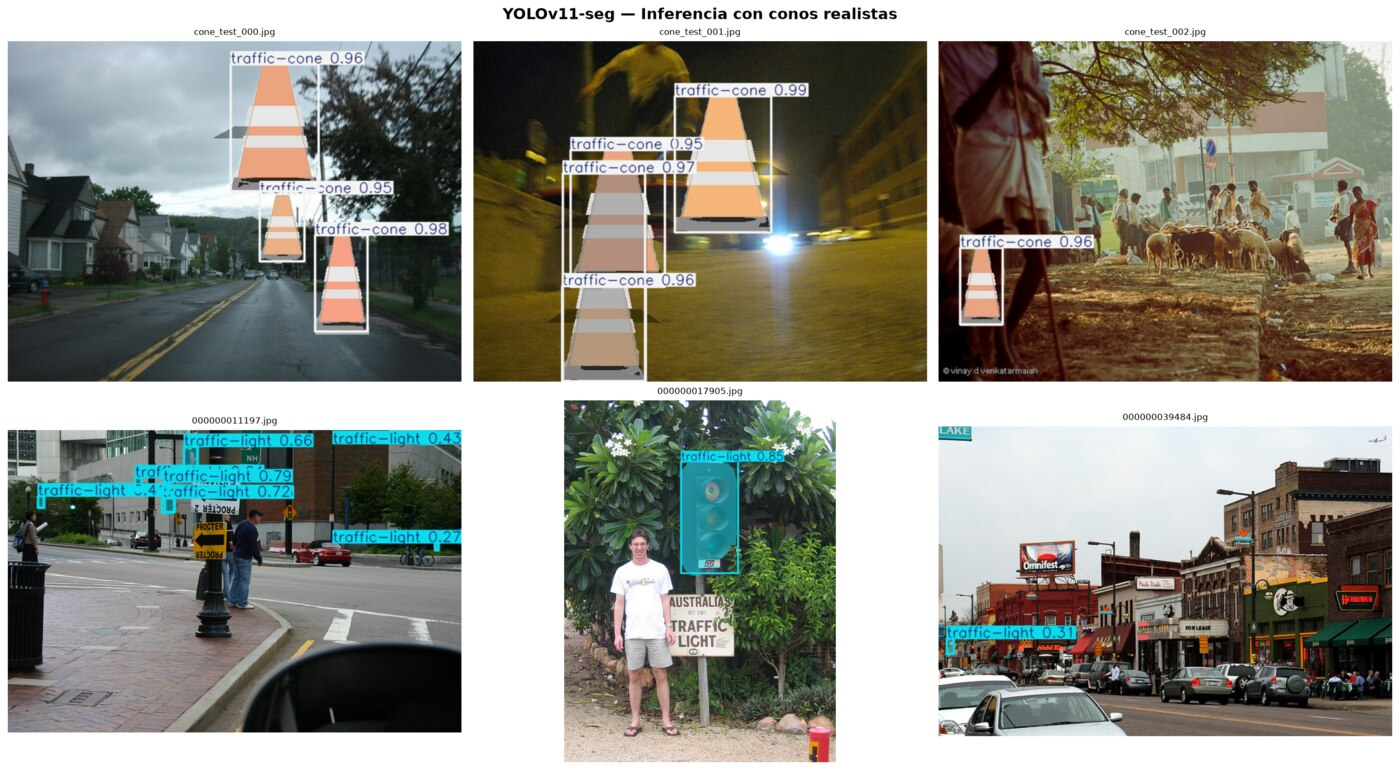
\includegraphics[width=0.85\textwidth]{capturas/inferencia_conos_realistas.png}
  \caption{Inferencia sobre conos de tránsito en fotografías reales (no sintéticas): el modelo generaliza correctamente pese a haber entrenado solo con conos sintéticos, con confianzas de 0.95 a 0.99.}
  \label{fig:inferencia_conos}
\end{figure}

\begin{figure}[htbp]
  \centering
  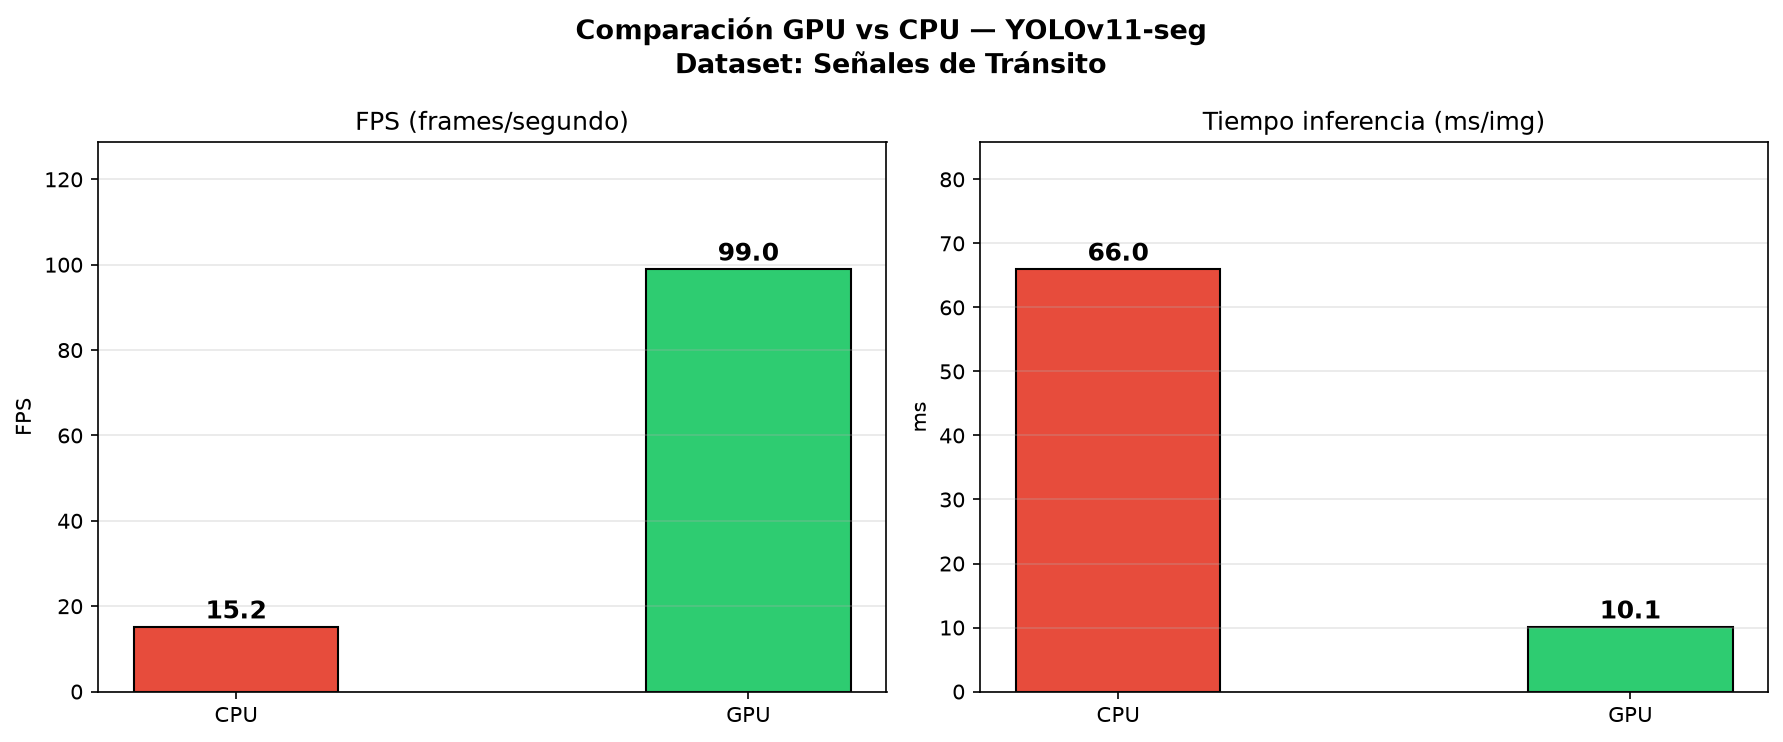
\includegraphics[width=0.7\textwidth]{capturas/benchmark_gpu_vs_cpu.png}
  \caption{Comparación GPU vs CPU de YOLOv11-seg sobre el dataset propio, RTX 3080 (50 inferencias).}
  \label{fig:benchmark1a}
\end{figure}

\begin{table}[htbp]
  \centering
  \caption{Benchmark GPU vs CPU -- Parte 1A (YOLOv11n-seg, RTX 3080)}
  \begin{tabular}{lccc}
    \toprule
    \textbf{Dispositivo} & \textbf{FPS} & \textbf{ms/img} & \textbf{Aceleración} \\
    \midrule
    CPU & 15.2 & 66.0 & -- \\
    GPU & 99.0 & 10.1 & 6.5x \\
    \bottomrule
  \end{tabular}
  \label{tab:benchmark1a}
\end{table}

Un dato interesante: el modelo generaliza a conos de tránsito reales (Figura~\ref{fig:inferencia_conos}) habiendo entrenado únicamente con conos sintéticos generados por OpenCV, lo que sugiere que la forma geométrica simple del cono (triángulo con franjas) es fácil de aprender incluso sin textura fotorrealista.

\textbf{Pendiente:} la guía pide segmentar imágenes capturadas por webcam en vivo, comparando GPU vs CPU. Dejamos lista la función \texttt{run\_webcam()} en el notebook, pero todavía no grabamos esa evidencia; queda pendiente para el equipo antes de la entrega final.

% =============================================================================
\section{Parte 1B: Detección YOLOv12/YOLOv26 y Super Resolución (individual)}
% =============================================================================

Esta parte la hice íntegramente en mi propio equipo (RTX 4060 Laptop, 7.65 GB VRAM, MAC \texttt{58:1c:f8:2e:dc:c7}), distinto al usado en la Parte 1A, conforme lo exige la guía que sea individual.

\subsection{Por qué RealPLKSR y no Real-ESRGAN}

La guía exige una red de super resolución de \textbf{no más de 2 años de existencia}. Real-ESRGAN (Wang et al., 2021)~[4] ya tiene alrededor de 5 años, así que la reemplacé por \textbf{RealPLKSR}~[3], una arquitectura CNN eficiente publicada en abril de 2024 (menos de 2 años a la fecha de esta práctica), pensada específicamente para super resolución de imágenes reales con degradaciones (ruido, blur, recompresión) -- el mismo caso de uso que cubría Real-ESRGAN. Usé los pesos públicos \texttt{4xNomosWebPhoto\_RealPLKSR} (licencia CC-BY-4.0), cargados con la librería \texttt{spandrel}.

\subsection{Metodología}

Construí dos scripts complementarios: \texttt{benchmark\_live.py}, pensado para grabar pantalla mostrando FPS, uso de RAM, salida de \texttt{nvidia-smi} y la dirección MAC del equipo en tiempo real; y \texttt{benchmark\_offline.py}, que corre el mismo benchmark de forma reproducible sobre imágenes fijas para tener números consistentes para este informe.

\begin{lstlisting}[style=pystyle]
def benchmark_detect(model_name, images, device, n=30):
    m = YOLO(MODELS[model_name])
    times = []
    for i in range(n):
        t0 = time.perf_counter()
        m(images[i % len(images)], device=device, verbose=False)
        times.append(time.perf_counter() - t0)
    return {'fps': 1/np.mean(times), 'ms': np.mean(times)*1000}
\end{lstlisting}

\subsection{Resultados}

\begin{table}[htbp]
  \centering
  \caption{Benchmark GPU vs CPU -- Parte 1B (RTX 4060 Laptop, 30 inferencias)}
  \begin{tabular}{llccc}
    \toprule
    \textbf{Tarea} & \textbf{Dispositivo} & \textbf{FPS} & \textbf{ms/img} & \textbf{Aceleración} \\
    \midrule
    YOLOv12n (detección)      & CPU & 19.7  & 50.7   & -- \\
    YOLOv12n (detección)      & GPU & 159.1 & 6.3    & 8.1x \\
    \midrule
    YOLOv26n (detección)      & CPU & 24.2  & 41.4   & -- \\
    YOLOv26n (detección)      & GPU & 209.4 & 4.8    & 8.7x \\
    \midrule
    RealPLKSR x4 (super res.) & CPU & 0.87  & 1152.0 & -- \\
    RealPLKSR x4 (super res.) & GPU & 20.61 & 48.5   & 23.7x \\
    \bottomrule
  \end{tabular}
  \label{tab:benchmark1b}
\end{table}

El uso de VRAM medido para RealPLKSR fue de \textbf{0.04 GB de 7.65 GB totales}, muy por debajo de la capacidad de la tarjeta, cumpliendo el requisito de la guía de verificar que la red no agote la memoria de video disponible.

La super resolución es la tarea que más se beneficia de la GPU (23.7x) porque es la más intensiva en cómputo por píxel (convoluciones de kernel grande sobre una imagen que además se \emph{aumenta} 4x); la detección se beneficia menos en términos relativos (8.1x--8.7x) porque YOLO nano ya es una arquitectura liviana pensada para correr razonablemente bien también en CPU.

\textbf{Pendiente:} la evidencia oficial que pide la guía es un \emph{vídeo en vivo} (no un benchmark offline) mostrando el overlay de FPS/RAM/\texttt{nvidia-smi}/MAC mientras corre \texttt{benchmark\_live.py} sobre webcam. Todavía tengo pendiente esa grabación antes de la entrega final; los números de esta sección son de una corrida offline reproducible sobre imágenes fijas, no de la grabación en vivo.

% =============================================================================
\section{Parte 1C: Pipeline OpenCV CUDA C++ -- CPU vs GPU-only (individual)}
% =============================================================================

Esta parte también es individual, y la hice en el mismo equipo (RTX 4060 Laptop) que la Parte 1B.

\subsection{Operaciones implementadas}

Implementé las cuatro operaciones que pide la guía -- suavizado Gaussiano, operaciones morfológicas (erosión/dilatación), detección de bordes (Canny) y ecualización de histograma -- en dos versiones: una con \texttt{cv::Mat} (CPU) y otra \emph{GPU-only} con \texttt{cv::cuda::GpuMat}, con un solo \texttt{upload()} al inicio y un solo \texttt{download()} al final para evitar transferencias intermedias CPU$\leftrightarrow$GPU.

\begin{lstlisting}
struct GpuPipeline {
    cv::Ptr<cv::cuda::Filter> gauss, erode_f, dilate_f;
    cv::Ptr<cv::cuda::CannyEdgeDetector> canny;

    explicit GpuPipeline(int type) {
        cv::Mat kernel = cv::getStructuringElement(cv::MORPH_ELLIPSE, cv::Size(3, 3));
        gauss = cv::cuda::createGaussianFilter(type, type, cv::Size(5, 5), 1.5);
        erode_f = cv::cuda::createMorphologyFilter(cv::MORPH_ERODE, type, kernel);
        dilate_f = cv::cuda::createMorphologyFilter(cv::MORPH_DILATE, type, kernel);
        canny = cv::cuda::createCannyEdgeDetector(50, 150);
    }
    cv::Mat process(const cv::Mat& frame, double& ms_total) {
        auto t0 = Clock::now();
        cv::cuda::GpuMat d_frame, d_gray, d_blur, d_eq, d_morph, d_edges;
        d_frame.upload(frame);
        cv::cuda::cvtColor(d_frame, d_gray, cv::COLOR_BGR2GRAY);
        gauss->apply(d_gray, d_blur);
        cv::cuda::equalizeHist(d_blur, d_eq);
        erode_f->apply(d_eq, d_morph);
        dilate_f->apply(d_morph, d_morph);
        canny->detect(d_morph, d_edges);
        cv::Mat result; d_edges.download(result);
        ms_total = elapsed_ms(t0);
        return result;
    }
};
\end{lstlisting}

\subsection{Un error de medición real y su corrección}

En la primera versión que escribí, los filtros CUDA (\texttt{createGaussianFilter}, \texttt{createMorphologyFilter}, \texttt{createCannyEdgeDetector}) se creaban dentro del ciclo de benchmark, en cada una de las 50 iteraciones. Eso hizo que la versión ``GPU'' midiera \textbf{más lenta} que la CPU (0.19x) -- un resultado que a primera vista parece un problema de rendimiento de la tarjeta, pero en realidad era un error mío de uso de la API: estas funciones son \emph{fábricas} pensadas para crearse una sola vez y reutilizarse con \texttt{->apply()} en cada frame. Al mover la creación de los filtros fuera del ciclo (estructura \texttt{GpuPipeline} de arriba), la GPU pasó a rendir por encima de la CPU, como cabía esperar.

\subsection{Resultados}

\begin{table}[htbp]
  \centering
  \caption{Benchmark CPU vs GPU-only -- Parte 1C (50 iteraciones, RTX 4060 Laptop)}
  \begin{tabular}{lccc}
    \toprule
    \textbf{Resolución} & \textbf{CPU (ms / FPS)} & \textbf{GPU-only (ms / FPS)} & \textbf{Aceleración} \\
    \midrule
    640$\times$640   & 0.81 / 1239.3 & 0.46 / 2151.4 & 1.74x \\
    1920$\times$1080 & 2.24 / 445.8  & 1.92 / 521.3  & 1.17x \\
    \bottomrule
  \end{tabular}
  \label{tab:benchmark1c}
\end{table}

\begin{figure}[htbp]
  \centering
  \begin{subfigure}[b]{0.3\textwidth}
    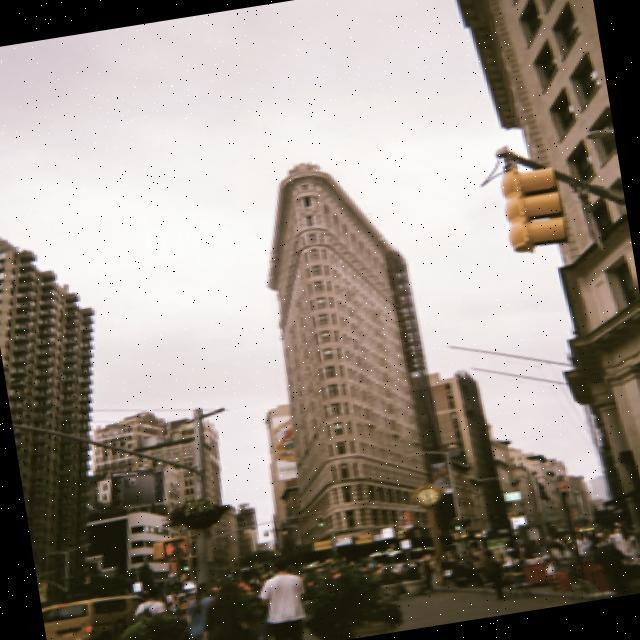
\includegraphics[width=\textwidth]{capturas/parte1c_original.jpg}
    \caption{Entrada original}
  \end{subfigure}
  \hfill
  \begin{subfigure}[b]{0.3\textwidth}
    
\includegraphics[width=\textwidth]{capturas/resultado_cpu.png}
    \caption{Pipeline CPU}
  \end{subfigure}
  \hfill
  \begin{subfigure}[b]{0.3\textwidth}
    
\includegraphics[width=\textwidth]{capturas/resultado_gpu.png}
    \caption{Pipeline GPU-only}
  \end{subfigure}
  \caption{Comparación cualitativa: los bordes detectados por CPU y GPU-only son visualmente idénticos, confirmando que la corrección del error de medición no alteró la lógica del pipeline.}
  \label{fig:parte1c}
\end{figure}

\subsection{Reflexión: pipeline CPU$\leftrightarrow$GPU vs GPU-only, y cuándo vale la pena la GPU}

Un pipeline que alterna CPU y GPU en cada operación (\texttt{upload}, procesar, \texttt{download}, procesar en CPU, volver a \texttt{upload}...) paga el costo de transferencia por el bus PCIe tantas veces como operaciones tenga. El pipeline GPU-only paga esa transferencia solo dos veces (una subida, una bajada), sin importar cuántas operaciones se encadenen en el medio.

Con solo cuatro operaciones livianas sobre imágenes de hasta 1080p, la ventaja de la GPU es real pero modesta (1.17x--1.74x): al ser pocas operaciones y relativamente baratas, el tiempo fijo de lanzar cada kernel CUDA representa una fracción considerable del tiempo total. La GPU empieza a valer claramente la pena cuando (a) el volumen de datos por frame crece (video de mayor resolución, procesamiento por lotes), (b) se encadenan más operaciones o más pesadas (por ejemplo, alimentar directamente una red neuronal CUDA con el resultado, como en la Parte 1B), evitando por completo el viaje de vuelta a CPU entre pasos, o (c) se necesita sostener una tasa de cuadros por segundo alta de forma prolongada, donde la CPU se satura por otras tareas del sistema y la GPU no.

% =============================================================================
\section{Conclusiones}
% =============================================================================

\begin{enumerate}

\item \textbf{La guía impone una restricción de individualidad real, no solo de forma.} Que la Parte 1A permita pareja y las Partes 1B/1C exijan un equipo y MAC distintos obliga a estructurar el proyecto en dos repositorios separados desde el principio, en vez de un solo entregable monolítico.

\item \textbf{Elegir una red por su ``novedad'' no es un detalle burocrático.} Real-ESRGAN sigue siendo una red de super resolución perfectamente funcional en 2026, pero ya no cumple el requisito de antigüedad de la guía. RealPLKSR (2024) resultó ser un reemplazo directo, compatible con la misma librería de carga (\texttt{spandrel}), sin tener que rediseñar el resto del pipeline.

\item \textbf{Un benchmark ``GPU pierde contra CPU'' es motivo de sospecha antes que de conclusión.} En la Parte 1C, el primer resultado (GPU 5x más lento) no reflejaba una limitación real de la tarjeta sino un uso incorrecto de la API de \texttt{cv::cuda} (crear filtros dentro del ciclo de medición). Vale la pena revisar el código de benchmark con la misma rigurosidad que el código de producción.

\item \textbf{La aceleración de GPU no es un número único: depende de la intensidad de cómputo de la tarea.} Super resolución (23.7x) se benefició mucho más que detección con YOLO nano (8.1x--8.7x), que a su vez se benefició más que un pipeline de 4 operaciones clásicas de bajo costo (1.17x--1.74x). A mayor trabajo por píxel, mayor ventaja relativa de la GPU.

\item \textbf{Verificar el consumo de VRAM es tan importante como verificar la velocidad.} RealPLKSR usó apenas 0.04 GB de los 7.65 GB disponibles en la RTX 4060 Laptop -- confirmar esto evita sorpresas de \texttt{out of memory} al escalar a resoluciones mayores o a un modelo más grande.

\end{enumerate}

% =============================================================================
\section*{Estado de la entrega y pendientes}
% =============================================================================

Este informe documenta el trabajo técnico completo (entrenamiento, benchmarks, código) hasta la fecha. Quedan dos pendientes de evidencia en vivo que la guía exige como grabación de vídeo, no como benchmark offline:

\begin{itemize}
  \item \textbf{Parte 1A (equipo):} grabar la segmentación en vivo por webcam, GPU vs CPU.
  \item \textbf{Parte 1B (individual):} grabar \texttt{benchmark\_live.py} en vivo (detección y super resolución, GPU vs CPU) mostrando el overlay de FPS/RAM/\texttt{nvidia-smi}/MAC.
\end{itemize}

% =============================================================================
\section*{Declaración de uso de herramientas de IA}
% =============================================================================

Parte del trabajo de esta práctica se apoyó en el modelo de inteligencia artificial \textbf{Claude Sonnet} (Anthropic, 2025), principalmente como asistente de programación y de redacción. En concreto ayudó a:

\begin{itemize}
  \item Escribir el script de fusión de datasets y la conversión de bounding boxes a polígonos rectangulares para entrenar segmentación, en una exploración individual previa mía sobre un dataset propio.
  \item Investigar y validar \textbf{RealPLKSR} como reemplazo de Real-ESRGAN, para cumplir el requisito de la guía de usar una red de super resolución de no más de 2 años de antigüedad.
  \item Depurar dos errores técnicos de la Parte 1C: un problema de configuración de CMake (el enlazado por defecto arrastraba módulos de OpenCV con símbolos rotos) y un error de medición en el pipeline GPU-only, donde los filtros CUDA se creaban dentro del ciclo de benchmark en lugar de una sola vez.
  \item Redactar este informe a partir de los resultados obtenidos en las ejecuciones reales de cada parte.
\end{itemize}

La lógica central de procesamiento de imágenes (transfer learning con YOLO, operaciones de \texttt{cv::cuda}, benchmarking GPU vs CPU) sigue directamente las formulaciones de la \textit{Guía de Práctica 4.1-4.2} del docente y el material teórico de la asignatura.

% =============================================================================
\section*{Referencias}
% =============================================================================

\begin{enumerate}[label={[\arabic*]}]
  \item Robles Bykbaev, V. (2026). \textit{Guía de Práctica de Laboratorio 4.1-4.2: Clasificación de Objetos Usando Técnicas de Deep Learning}. Universidad Politécnica Salesiana.

  \item Jocher, G., et al. (2024). \textit{Ultralytics YOLO Docs} (v11/v12/v26). \url{https://docs.ultralytics.com}.

  \item Lee, D., Yun, S., \& Ro, Y. (2024). Partial Large Kernel CNNs for Efficient Super-Resolution. \textit{arXiv:2404.11848}.

  \item Wang, X., et al. (2021). Real-ESRGAN: Training Real-World Blind Super-Resolution with Pure Synthetic Data. \textit{ICCVW 2021}.

  \item chaiNNer-org. (2025). \textit{Spandrel — PyTorch architecture library for super-resolution}. \url{https://github.com/chaiNNer-org/spandrel}.

  \item Bradski, G., \& Kaehler, A. (2008). \textit{Learning OpenCV: Computer Vision with the OpenCV Library}. O'Reilly Media.

  \item NVIDIA Corporation. (2025). \textit{OpenCV CUDA Module Documentation}. \url{https://docs.opencv.org}.

  \item Lin, T.Y., et al. (2014). Microsoft COCO: Common Objects in Context. \textit{ECCV 2014}.

  \item Anthropic. (2025). \textit{Claude Sonnet — AI assistant}. \url{https://www.anthropic.com}. \textit{[Asistencia en scripts de datos, depuración de CUDA/CMake e investigación de RealPLKSR]}
\end{enumerate}

\end{document}
